\begin{frame}
\frametitle{Machine Learning Review}

\resizebox{!}{0.8\paperheight}{
\begin{tikzpicture}
    [ node distance = 0.15in
    ]
    \Large

\node
    [ inner sep=0
    ] (img) 
    {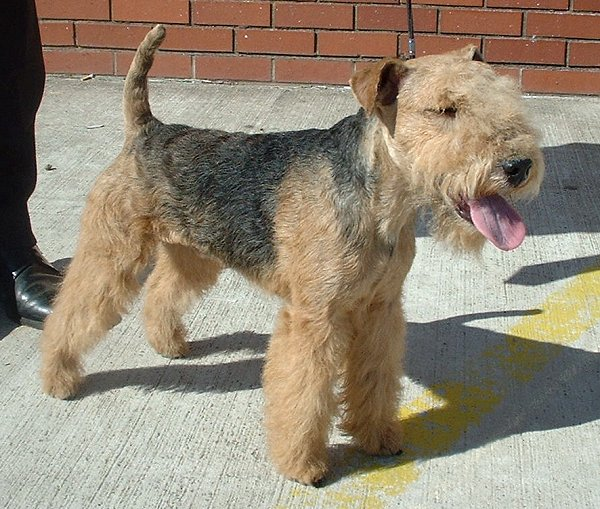
\includegraphics[width=3in]{img/Lakeland_Terrier}};

\uncover<1-3>{
\node
    [ below = of img
    , anchor=north
    , fill=darkgray
    , minimum height=1.15in
    , minimum width=3in
    , align=center
    , text centered
    , inner sep=0
    ]
    { \color{white} Machine Learning Model };
}

\uncover<4->{
\node 
    [ below = of img
    , anchor=north
    , fill=darkgray
    , minimum width=3in
    , minimum height=0.5in
    , align=center
    , inner sep=0
    , outer sep=0
    ](features)
    {\color{white}\centering Feature Generation};

\node
    [ below = of features
    , draw
    , text width = 3in
    , minimum height= 0.5in
    , align=center
    , inner sep=0
    , outer sep=0
    ](xentropy)
    {\parbox{\textwidth}{\centering Logistic Regression}};
\draw[->,line width=2pt] (features) -- (xentropy);
}

\uncover<1->{
\node
    [ below = 0.2in of xentropy
    , inner sep=0.1in
    , text width=2.8in
    , draw
    ]
    (classes)
    {
        %Class Predictions:
        %\vspace{0.1in}
        \begin{tikzpicture}
        %\small
        \tt
        \foreach  \l/\x[count=\y] in 
            { not-animal/4
            , animal/96
            }
        {\node[left,text width=1.0in] at (0,0.8*\y) {\l~~};
        \draw[draw=blue,fill={rgb,255:red,170; green,170; blue,255}] (0.0,0.8*\y-.3) rectangle (0.0+\x/100.0*3,0.8*\y+.3);
        \node[right] at (0.0+\x/100.0*3,.8*\y) {\x\!\%};
        }
        \end{tikzpicture}
    };
}

\draw[->,line width=2pt] (img) -- (features) ;
\draw[->,line width=2pt] (xentropy) -- (classes);

%%%%%%%%%%%%%%%%%%%%


\uncover<5,6>{
\node
    [right = 0.25in of features
    , text width = 5in
    ]
    (deep_place) {};

\node
    [ above = -2.0in of deep_place
    , text width = 5in
    ] (deep) {
    \baselineskip=16pt
    Highly domain specific\\
    ~\\
    \emph{Deep Learning} is state-of-the-art for images/text \\
    ~\\
    Lots of famous \emph{network architectures}:\\
    ~~~~LeNet \citep{lecun1998gradient} \\
    ~~~~AlexNet \citep{krizhevsky2012imagenet} \\
    ~~~~VGG \citep{simonyan2014very} \\
    ~~~~Inception v1 \citep{szegedy2015going} \\
    ~~~~Inception v2 \citep{ioffe2015batch} \\
    ~~~~Inception v3 \citep{szegedy2016rethinking} \\
    ~~~~Inception v4 \citep{he2016identity} \\
    ~~~~ResNet \citep{witten2016data} \\
    ~~~~ResNet2 \citep{he2016identity} \\
    %~~~~WideResNet \citep{zagoruyko2016wide} \\
    %~~~~SqueezeNet \citep{iandola2016squeezenet} \\
    ~~~~MobileNet \citep{howard2017mobilenets} \\
    ~~~~DenseNet \citep{huang2017densely} \\
    ~~~~ResNext \citep{lin2018focal} \\
    ~~~~NASNet \citep{zoph2018learning} \\
    ~~~~PNASNet \citep{liu2018progressive} \\
    %~~~~SqueezeExcitationNet \citep{hu2018squeeze} \\
    %~~~~MobileNet2 \citep{sandler2018mobilenetv2} \\
    ~~~~... \emph{and many more} ... \\
    ~\\
    \textbf{No theoretical guarantees}
    };
    \draw [decorate,decoration={brace,mirror,amplitude=10pt,raise=4pt, aspect=0.6},yshift=0pt]
        (deep.north west) -- (deep.south west) node [black,midway,anchor = west,xshift=0.8cm] {};
    }

%\uncover<6>{\node at (3.5in,-3.25in) [ text width = 5in,align=center ] {\textbf{better than Humans in practice} };}
%\uncover<6>{\node at (3.5in,-3.5in) [ text width = 4in,align=center ] {\textbf{treat as black box} };}
%
%\uncover<7->{
%\node
    %[ right = 0.25in of features
    %, text width = 3in
    %] (rd) {
        %Outputs a vector $\R^d$, $d$ is the number of features
    %};
    %}

\uncover<8->{
\node
    [ right = 0.25in of xentropy
    , text width = 6in
    ] (deep) {
        \baselineskip=16pt
        ~\\
        Known since the 1800s, good theoretical properties\\
        \vspace{0.15in}
        Let $d$ be number of features,\\
        \hspace{0.33in}$k$ be number of classes,\\
        \hspace{0.33in}$n$ be number of data points,\\
        then the generalization error = $\Theta\left(\sqrt{\frac{kd}{n}}\right)$
        \\
        \vspace{0.15in}
        \textbf{So more classes requires more data}
        ~\\
        %Known since at least \citet{nelder1972generalized}
    };
    \draw [decorate,decoration={brace,mirror,amplitude=10pt,raise=4pt},yshift=0pt]
        (deep.north west) -- (deep.south west) node [black,midway,anchor = west,xshift=0.8cm] {};
};
\end{tikzpicture}
}
\end{frame}
